

\section{Getting started}
\subsection{Obtaining access authorization / Requesting a new password}

% Die Zugangsberechtigung zum CUBE PA erhalten Sie für das Projekt Zugkunft Waldenburgerbahn beim Gesamtleiter. Senden Sie
% eine E-Mail an folgende Adresse (Zeitpunkt der Aufschaltung wird noch bekanntgegeben):

The access authorization to CUBE PA is given to you by the project manager. If you have questions about the responsibilities or the release of a CUBE PA access, send an e-mail to the following address:

\vspace{\baselineskip}

% \href{mailto:cube.support@emchberger.ch}{\textstyleInternetlink{cube.support@emchberger.ch}}
{\color{red} cube.support@emchberger.ch}

\vspace{\baselineskip}

If you have forgotten your password, you can request a new one on the login page of CUBE PA using the 'Forgot password' function. A link to reset your password will be sent to you by e-mail.If you have questions you can also contact the above e-mail address.

\vspace{\baselineskip}

For safety reasons we recommend that you immediately change passwords received by e-mail.

\subsection{Internet connection}

A functioning Internet connection is a prerequisite for using CUBE PA. Working offline is not supported, as all data is saved on a server.

\vspace{\baselineskip}

If you experience unexpected problems while using CUBE PA, check the status symbol of the connection in the lower right corner of the screen. A red symbol indicates that the Internet connection is interrupted. If this happens while you are entering data, try to restore the Internet connection, and then click 'Update' to back up the data in the local memory of CUBE PA.
If you are unable to quickly re-establish the Internet connection, do not exit CUBE ProjectAssistant or turn off the computer. Find another location where you can establish an Internet connection and as soon as you have one, click on 'Update'.

\vspace{\baselineskip}

\textbf{Connection status:}

\vspace{\baselineskip}

\begin{tabular}{c | p{14cm} l} %{cl}

\vspace{+1pt}	

\includegraphics[height=12pt] {/Icons/online.jpg} & You have an Internet connection and you are logged in to CUBE PA. \\
\vspace{+1pt}	

\includegraphics[height=12pt]{/Icons/offline.jpg} & The Internet connection is interrupted or the CUBE PA server is temporarily unavailable. \\
\vspace{+1pt}	

\includegraphics[height=12pt]{/Icons/abgemeldet.jpg} & No status symbol is visible. You have an Internet connection but you are not logged in to CUBE PA. \\

% 
\includegraphics[height=12pt]{/Icons/BlaueWolke_Blitz.jpg} & Sie haben eine Internet-Verbindung, sind aber nicht in CUBE PA angemeldet \\

\end{tabular}

\vspace{\baselineskip}

If you exit CUBE PA while the Internet connection is interrupted, the data entered last will be lost.

\subsection{Starting CUBE PA}

% Benutzerspezifisch

CUBE PA can be accessed at the following address:

\vspace{\baselineskip}

{\color{red} http://www.cubetools.ch/}

\vspace{\baselineskip}

You are directed to the CUBE Tools start page:

\begin{figure}[H]
\center{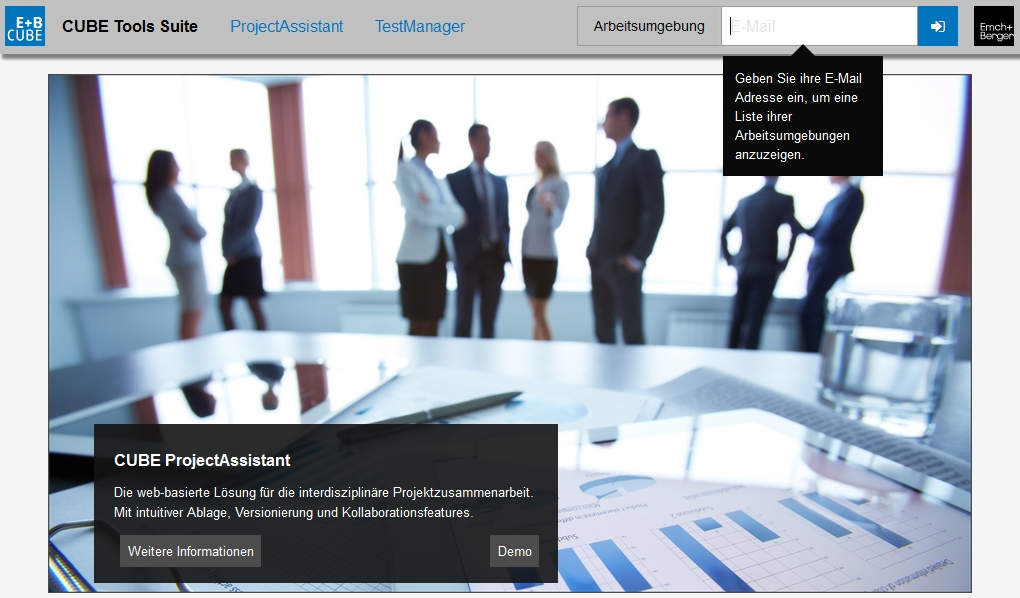
\includegraphics[width=1\linewidth]{../chapters/02_GettingStarted/pictures/2-3_Einstiegsseite.jpg}}
\caption{The CUBE Tools start page}
% \label{fig:speciation}
\end{figure}

Enter your e-mail address at the top right corner of the screen and click on the blue arrow button next to it:

\begin{figure}[H]
\center{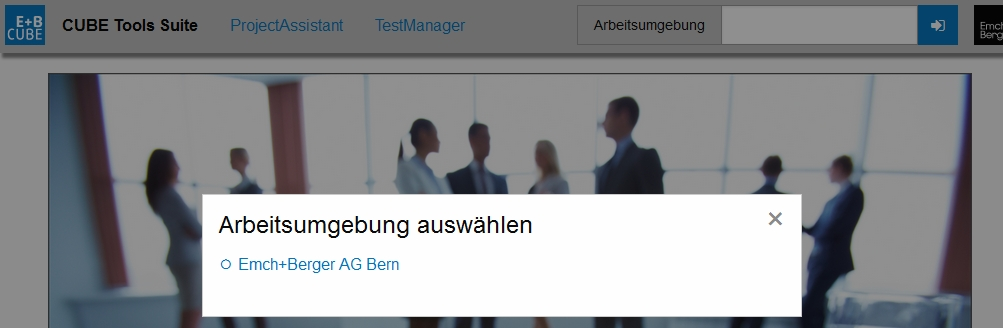
\includegraphics[width=1\linewidth]{../chapters/02_GettingStarted/pictures/2-3_Arbeitsumgebung_auswaehlen.jpg}}
\caption{Workspace choice}
% \label{fig:speciation}
\end{figure}

All workspaces in which you are registered will be shown. Click on the desired workspace. You are directed to the log-in form:

\begin{figure}[H]
\center{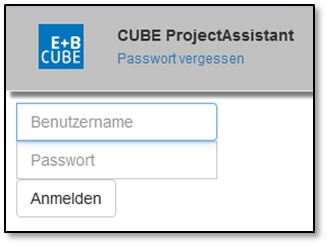
\includegraphics[width=0.35\linewidth]{../chapters/02_GettingStarted/pictures/2-3_CUBEPA_Anmeldung.jpg}}
\caption{Logging in to CUBE PA}
% \label{fig:speciation}
\end{figure}

Enter your username and your password. When you click on 'Log in', your personal overview appears.

\vspace{\baselineskip}

\textbf{Note:} If your valid login details are already in the browser (e-mail address and password), you will be directly logged in to CUBE PA.

\subsection{Changing the password}
\label{bkm:Ref434828103}

For safety reasons we recommend that you immediately change any password received by e-mail. To do so, click on your name in the upper left corner of the screen. A menu appears, allowing you to log out from CUBE PA, change your password, or open or save this user manual.

\begin{figure}[H]
\center{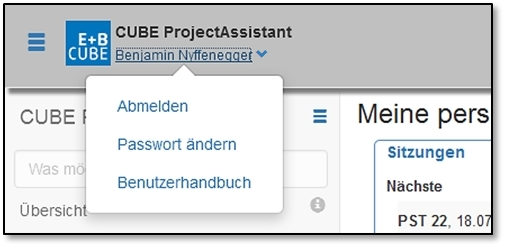
\includegraphics[width=0.5\linewidth]{../chapters/02_GettingStarted/pictures/2-4_Passwort_aendern.jpg}}
\caption{Changing the password}
% \label{fig:speciation}
\end{figure}

By clicking on 'Change password' a form appears, in which you need to enter your old password once and your new password twice:

\begin{figure}[H]
\center{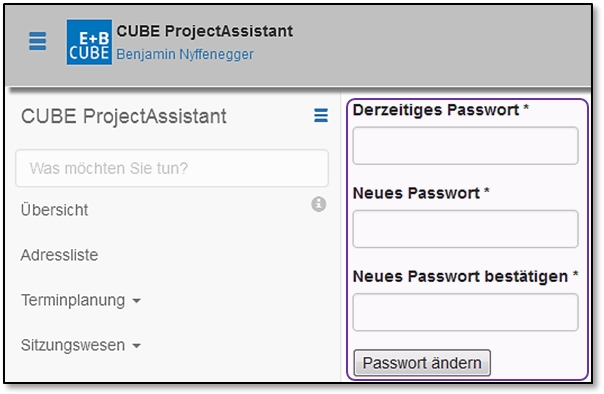
\includegraphics[width=0.5\linewidth]{../chapters/02_GettingStarted/pictures/2-4_Passwort_Eingabe.jpg}}
\caption{Setting a new password}
% \label{fig:speciation}
\end{figure}

As soon as you click on the 'Change password' button, the new password becomes valid.

\subsection{The most important menus, buttons and symbols briefly explained}

The CUBE PA operation is oriented towards usual Internet application operation. If you regularly use a smartphone or a tablet, you will quickly find your way in CUBE PA.

\vspace{\baselineskip}

This chapter gives an overview of the most important menus, buttons and symbols, which appear in all parts of CUBE PA and always have the same meaning.

\pagebreak

\subsubsection{Menus}

\begin{figure}[H]
\center{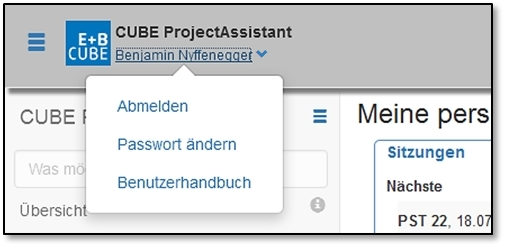
\includegraphics[width=0.5\linewidth]{../chapters/02_GettingStarted/pictures/2-4_Passwort_aendern.jpg}}
\caption{The start-up menu}
% \label{fig:speciation}
\end{figure}


The name of the user currently logged in to CUBE PA appears at the top left. Click on the name to display more options. The password changing option was described above (Chapter \ref{bkm:Ref434828103}). Click on 'User Manual' to open this manual as a PDF file or to save it. Click on 'Log out' to directly exit CUBE PA. If you have unsaved data, a warning appears.

\begin{figure}[H]
\center{\includegraphics[width=1\linewidth]{../chapters/02_GettingStarted/pictures/251_Browsermeldung.jpg}}
\caption{Browser warning}
% \label{fig:speciation}
\end{figure}
\begin{small}
The content of this message depends on the used browser (in this case, Firefox) and therefore cannot be influenced.
\end{small}

\vspace{\baselineskip}

You can cancel exiting CUBE PA (Stay on page) and save the unsaved data by clicking on 'Update'.

\vspace{\baselineskip}

\pagebreak

The main menu is located on the left:

\vspace{\baselineskip}

\begin{wrapfigure}[20]{l}{6.5cm}   % [x] Wie manche Zeile soll sich um die Grafik "brechen"
  \vspace{-35pt}      % Grundwert war 20; mit 30 schön oben beim Text ausgerichtet
  \begin{center}
    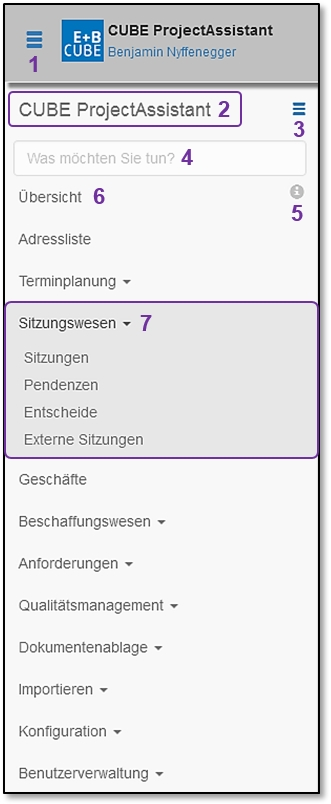
\includegraphics[width=1\linewidth]{../chapters/02_GettingStarted/pictures/2-5-1_Menu_Uebersicht.jpg}
  \end{center}
  \vspace{-20pt}
  \caption{Using the menu}
  \vspace{-10pt}
\end{wrapfigure}

The menu enables you to choose from different fields to which you have authorized access. Depending on your authorizations, your menu may differ from this image. Menu subcategories (in this case for example 'External Meetings' under Meeting Management) may differ, as menu items can be configured specifically for a customer. The basic functions are however the same. By clicking on the menu icon \col{(1)} you can show and hide the entire menu. This gives you additional workspace in your browser when needed. \\
The designation under \col{(2)} shows you the current workspace. By clicking on the icon \col{(3)} you can directly switch between workplaces.

\vspace{\baselineskip}

\begin{raggedleft}
\hspace{80mm} 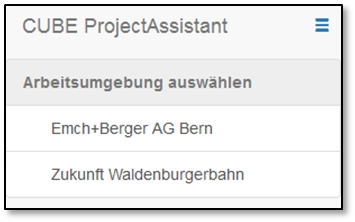
\includegraphics[height=40mm]{../chapters/02_GettingStarted/pictures/2-5-1_Arbeitsumgebung_wechseln.jpg}
\end{raggedleft}

\vspace{\baselineskip}

You will only see workspaces to which you have authorization. Click on the desired workspace to go to its log in window. If you had already opened a workspace on the same day (without restarting the computer), you can return to the desired workspace without logging in. Click again on the icon \col{(3)} to close the workspace selection. 

\vspace{\baselineskip}

A central tool is the 'What would you like to do?' search filed \col{(4)}. The info-icon \col{(5)} provides useful information for a productive and effective search:

\begin{figure}[H]
\center{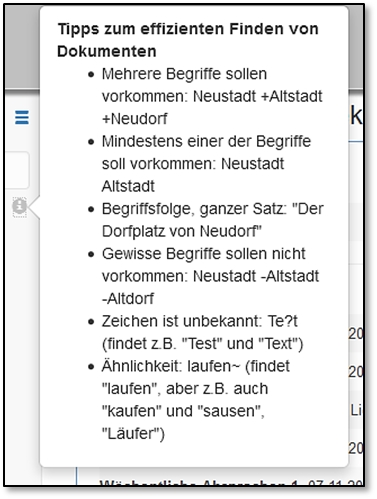
\includegraphics[width=0.35\linewidth]{../chapters/02_GettingStarted/pictures/2-5-1_Hilfe_zu_Suche.jpg}}
\caption{Tips for an effective search}
% \label{fig:speciation}
\end{figure}

Click anywhere in the browser window to close the info-window. Enter the desired term/s in the search field \col{(4)}. CUBE PA searches all menu fields and entries, as well as contents of uploaded documents (for example Word and PDF documents). \\

\textbf{It is important to note} that PDF documents can only be searched if they consist of integrated text and not images. If a text is scanned and saved as an image in a PDF file, its contents will not be searched.\\

\begin{wrapfigure}[14]{r}{7cm}   % [x] Wie manche Zeile soll sich um die Grafik "brechen"
  \vspace{-30pt}      % Grundwert war 20; mit 30 schön oben beim Text ausgerichtet
  \begin{center}
    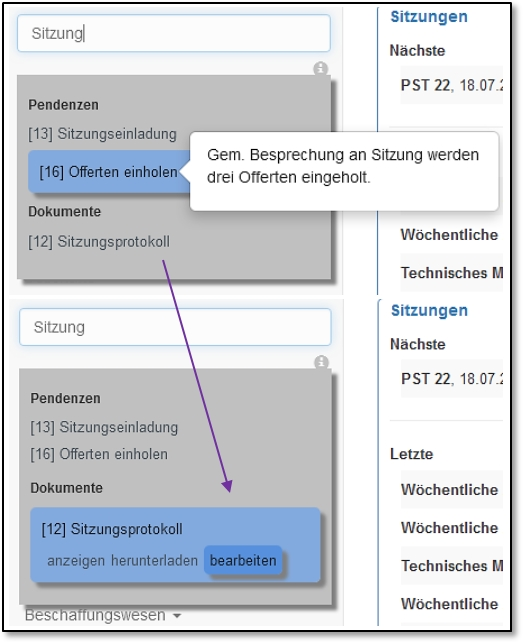
\includegraphics[width=0.8\linewidth]{../chapters/02_GettingStarted/pictures/2-5-1_Such_Ergebnisse.jpg}
  \end{center}
  \vspace{-20pt}
  \caption{Using search results}
  \vspace{-10pt}
\end{wrapfigure}

All found matches are now displayed:

\begin{compactitem}
	\item Under the keyword you can find entries in actions and in documents.
	\item Hover over an entry in the actions and the details of that entry are displayed.
	\item Under other fields, in this case under documents, you can show, download, or edit a document (a meeting document in this example). To do so, hover the mouse over the desired document and click on the desired option.
\end{compactitem}

\vspace{\baselineskip}

The menu item 'Dashboard' \col{(6)} always redirects you to your personal overview. When subcategories are available under a menu item, for example under 'Meeting Management', a small triangle is shown. Click on the item to display the corresponding subcategories \col{(7)}. The main item 'Meeting Management' is itself not linked. Click on it again to close the subcategories.

\vspace{\baselineskip}

The main menu gives access to the different CUBE PA fields. Depending on user access authorizations, not all fields are visible and accessible for all users.

\begin{itemize}
\item
\textbf{Dashboard}: View of meetings, actions, documents and procurements which are relevant to you.
\item
\textbf{Address List}: View of the addresses with a filter function. New entries (persons and organizations) can also be made here.
\item
\textbf{Scheduling}: View and editing of schedules.
\item
\textbf{Meeting Management}: View and editing of meetings, meeting minutes, actions and 
decisions.
\item
\textbf{Procurement Function}: Procurements process, from the call for tenders to the contract conclusion.
\item
\textbf{Requirements}: Access to documents with requirements.
\item
\textbf{Quality Management}: Access to documents about risk management and interfaces. The project handbook and other handbooks can also be compiled here.
\item
\textbf{Document Management}: Document management with online view. Modified documents are archived with new version numbers.
\item
\textbf{Import}: Data import (projectplans and transactions).
\item
\textbf{Configuration}: Definition and management of selection list contents.
\item
\textbf{User Management}: User, team and group administration.
\end{itemize}

% bishierher

\subsubsection{Buttons}

The following buttons are always used:

\vspace{\baselineskip}

% 2.8, 12

\begin{tabular}{|c | p{10cm}|l} %{cl}
\hline
\raisebox{-1\totalheight}{
\includegraphics[height=20pt]{/Icons/B_Erstellen.jpg}} & Create: By clicking on this button you save a new data record for the same time, with the possibility of further editing it. \\
\hline
\raisebox{-1\totalheight}{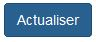
\includegraphics[height=20pt]{/Icons/B_Uebernehmen.jpg}} & Update: By clicking on this button, recently entered or recently modified data, which so far only exists in your computer's memory, is backed up on the server. \\
\hline
\raisebox{-1\totalheight}{
\includegraphics[height=20pt]{/Icons/Lupe_s.jpg}} & Magnifying Glass: By clicking on this magnifying glass, a list is filtered out based on the filter criteria you have selected or the search term you have entered in the fields on the first line of the list. \\
\hline
\raisebox{-1\totalheight}{
\includegraphics[height=20pt]{/Icons/FilterLoeschen.jpg}} & Delete filter: By clicking on this symbol, all entries in the search fields are deleted. \\
\hline
\raisebox{-1\totalheight}{
\includegraphics[height=20pt]{/Icons/Blattsymbol_s.jpg}} & Dog-eared sheet: By clicking on this button, a PDF file of the list with the current filter settings is generated. When no filter is applied, the entire list is generated as a PDF file. \\
\hline
\raisebox{-1\totalheight}{
\includegraphics[height=16pt]{/Icons/weitereSeiten.jpg}} & Pagination: With these buttons you can move forwards or backwards within a list by clicking on 'Next' or 'Previous' or by clicking on a specific page number. When a list has more than five pages, not all page numbers are displayed. Click on 'Next' or 'Previous' until the desired pages can be selected. \\
\hline
\end{tabular}

\begin{figure}[H]
\center{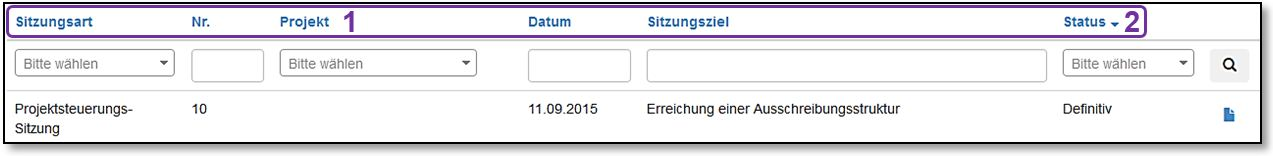
\includegraphics[width=1\linewidth]{252_Listen_sortieren.jpg}}
\caption{Columns: Sorting content}
% \label{fig:speciation}
\end{figure}


Additionally, all list column titles highlighted in blue work as buttons \col{(1)}. By clicking on a column title, the list is sorted in ascending order according to this column. By clicking again on the column title, the order is inverted. 
The small triangle 
\includegraphics[height=10pt]{/Icons/welcheSpalte_sort.jpg} \col{(2)} shows according to which column the list is sorted (in this example according to 'Archive Status') and in which order it is sorted: (Sorting A {\textgreater} Z 
\includegraphics[height=10pt]{/Icons/Status_down.jpg} or Z {\textgreater} A 
\includegraphics[height=10pt]{/Icons/Status_up.jpg}).

\pagebreak
\subsubsection{Symbols}
\label{bkm:Ref443039356}
The following symbols have the same meaning all over CUBE PA. Such buttons and text links generally change color when the mouse pointer is hovered over them. (This does not apply to the connection status symbol). 

\begin{tabular}{|c|p{14cm}|} %{cl}
\hline
\raisebox{-0.5\totalheight}{
\includegraphics[height=12pt]{/Icons/online.jpg}} & These green arrows appear at the bottom right of the window. They indicate that you have an Internet connection and that you are logged in to CUBE PA. \\

\includegraphics[height=12pt]{/Icons/offline.jpg} & If these arrows are red, this means that the Internet connection is interrupted or that the CUBE PA server is temporarily unavailable. \\

\includegraphics[height=12pt]{/Icons/abgemeldet.jpg} & If you don't see the arrows, it means that you are not currently logged in to any CUBE PA workspace. \\
\hline
\raisebox{-1\totalheight}{
\includegraphics[height=12pt]{/Icons/Plussymbol.jpg}} & This plus (new) symbol appears in the top left corner of a window. Clicking it enables you to create a new data record (for example, a new meeting). \\
\hline
\raisebox{-1\totalheight}{
\includegraphics[height=12pt]{/Icons/Filter.jpg}} & Clicking on the filter symbol displays advanced filter options. These filter settings can be saved and later modified. \\
\hline
\raisebox{-1\totalheight}{
\includegraphics[height=12pt]{/Icons/Nadelsymbol.jpg}} & Click on the pin symbol to show or hide the Google Maps overview. \\
\hline
\raisebox{-1\totalheight}{
\includegraphics[height=12pt]{/Icons/Listensymbol_zurueck.jpg}} & Clicking the list (repository) symbol brings you back to the overview. This symbol usually appears when you are in a specific data record after having used the magnifying glass symbol (show) or the pen symbol (edit). \\
\hline
\raisebox{-1\totalheight}{
\includegraphics[height=12pt]{/Icons/SpaltenEinst.jpg}} & Clicking on this configuration symbol allows you to add or remove certain columns in the list. Unneeded columns can be deselected. \\
\hline
\raisebox{-1\totalheight}{
\includegraphics[height=12pt]{/Icons/Stift.jpg}} & The pen symbol is usually in the left corner near a field in a list. Clicking on it enables you to edit the contents of this field.   
\includegraphics[height=14pt]{253_Datum_edit.jpg}\\
\hline
\raisebox{-1\totalheight}{
\includegraphics[height=12pt]{/Icons/Bearbeiten.jpg}} & Pen in square (small): By clicking on this (edit) symbol a form is opened, which allows you to edit all the fields of the selected data record. \\
\hline
\raisebox{-1\totalheight}{
\includegraphics[height=12pt]{/Icons/Pluszeichen.jpg}} & Plus sign: By clicking on this plus sign (Add), you can add a new entry to a list. For example, you can add an additional participant to a meeting. \\
\hline
\raisebox{-1\totalheight}{
\includegraphics[height=12pt]{/Icons/Lupe.jpg}} & Magnifying glass: This (show) symbol is found directly next to a line / entry in a list. By clicking on it a form is opened, which allows you to view all the fields of the selected data record. \\
\hline
\raisebox{-1\totalheight}{
\includegraphics[height=12pt]{/Icons/Blattsymbol.jpg}} & Dog-eared sheet: This symbol appears in a list field. Clicking on it generates a PDF file. The column title determines the contents of the PDF document. \\
\hline
\raisebox{-1\totalheight}{
\includegraphics[height=12pt]{/Icons/VertPfeile.jpg}} & Opposing vertical arrows: This symbol allows you to change the position of an entry within a list. Click and hold the symbol to drag the entry and drop it in the desired position. \\
\hline
\raisebox{-1\totalheight}{
\includegraphics[height=12pt]{/Icons/Muelltonne.jpg}} & Garbage bin: Clicking on this (remove) symbol deletes a row from a list as well as all data belonging to it. For example, it deletes the information of an attachment and the attachment itself. A security message „Remove?“ appears. By conforming with „OK“ the data is deleted. \\
\hline
\raisebox{-1\totalheight}{
\includegraphics[height=12pt]{/Icons/Kreuzchen.jpg}} & Crosses in fields: Clicking on a cross in the right side of a field clears the contents of a field with a selection list. \\
\hline
\raisebox{-1\totalheight}{
\includegraphics[height=12pt]{/Icons/Pfeil_rechts.jpg}} & Horizontal arrow symbol: Clicking on it shows the content (makes it visible). \\
\hline
\raisebox{-1\totalheight}{
\includegraphics[height=12pt]{/Icons/Pfeil_unten.jpg}} & Vertical arrow symbol: Clicking on it hides the content (makes it invisible). \\
\hline
\end{tabular}

\subsubsection{Warnings and tips}
If you fill in data fields in CUBE PA without clicking on 'Update' or 'Create' and decide to leave the current page, the following message appears: 

\begin{figure}[H]
\center{\includegraphics[width=1\linewidth]{251_Browsermeldung.jpg}}
\caption{Browser warning}
% \label{fig:speciation}
\end{figure}
\begin{small}
The content of this message depends on the used browser (here Firefox) and therefore cannot be influenced.
\end{small}

\vspace{\baselineskip}

You have the possibility of clicking on 'Stay on page' and then on 'Update' to back up the data. The data will otherwise be lost.

\vspace{\baselineskip}

When entering data, there are mandatory fields which must be filled out. If a mandatory field is left empty, the following message appears:

\begin{figure}[H]
\center{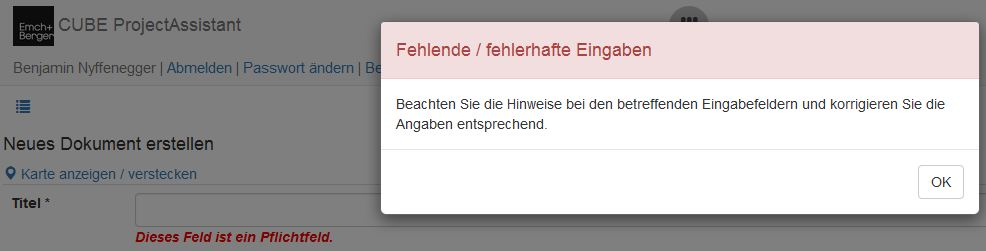
\includegraphics[width=1\linewidth]{254_WarnungPflichfelder}}
\caption{Mandatory field warning}
% \label{fig:speciation}
\end{figure}

The mandatory field that must be filled out is indicated with 'This field is required' in red. The warning can be removed by clicking on 'OK'. Saving the data becomes possible after the mandatory field is filled out. 


\subsection{CUBE PA on mobile devices (Smartphones, Tablets)}

CUBE PA can also be used on mobile devices such as smartphones and tablets. CUBE PA recognizes that it's on a mobile device and automatically switches to the 'mobile' view. This includes a slightly different display as well as adapted menu navigation (see below). However, if you are working with tablets on which a regular Windows operating system is installed (for example, Win 8.1 / Win 10 on Microsoft Surface), the view will not be changed, and CUBE PA cannot be operated at all or only with touch inputs.


\begin{figure}[H]
\center{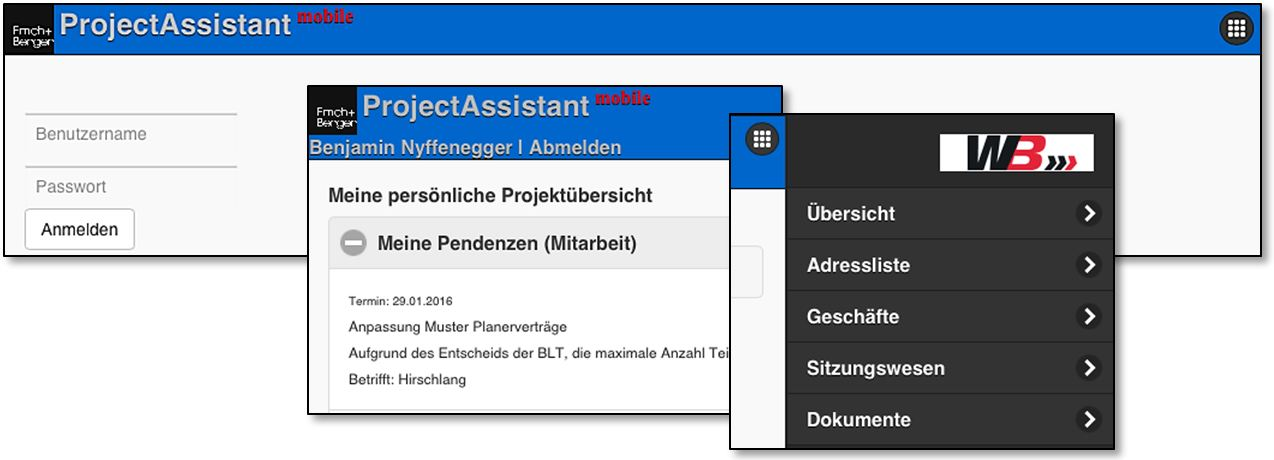
\includegraphics[width=1\linewidth]{26_Mobile_Ansicht.jpg}}
\caption{CUBE PA - mobile view}
% \label{fig:speciation}
\end{figure}

\vspace{\baselineskip}

\begin{tabular}{p{7cm} l} %{cl}
CUBE PA on an iPad: \newline Customized menu and selection \newline window for touch inputs. & \raisebox{-.6\totalheight}{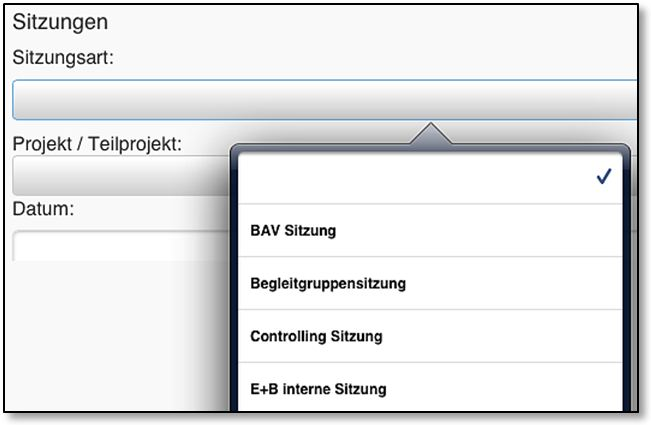
\includegraphics[width=.5\linewidth]{26_iPad_Sitzungen.jpg}}\\
\end{tabular}

\vspace{\baselineskip}

\begin{figure}[H]
\center{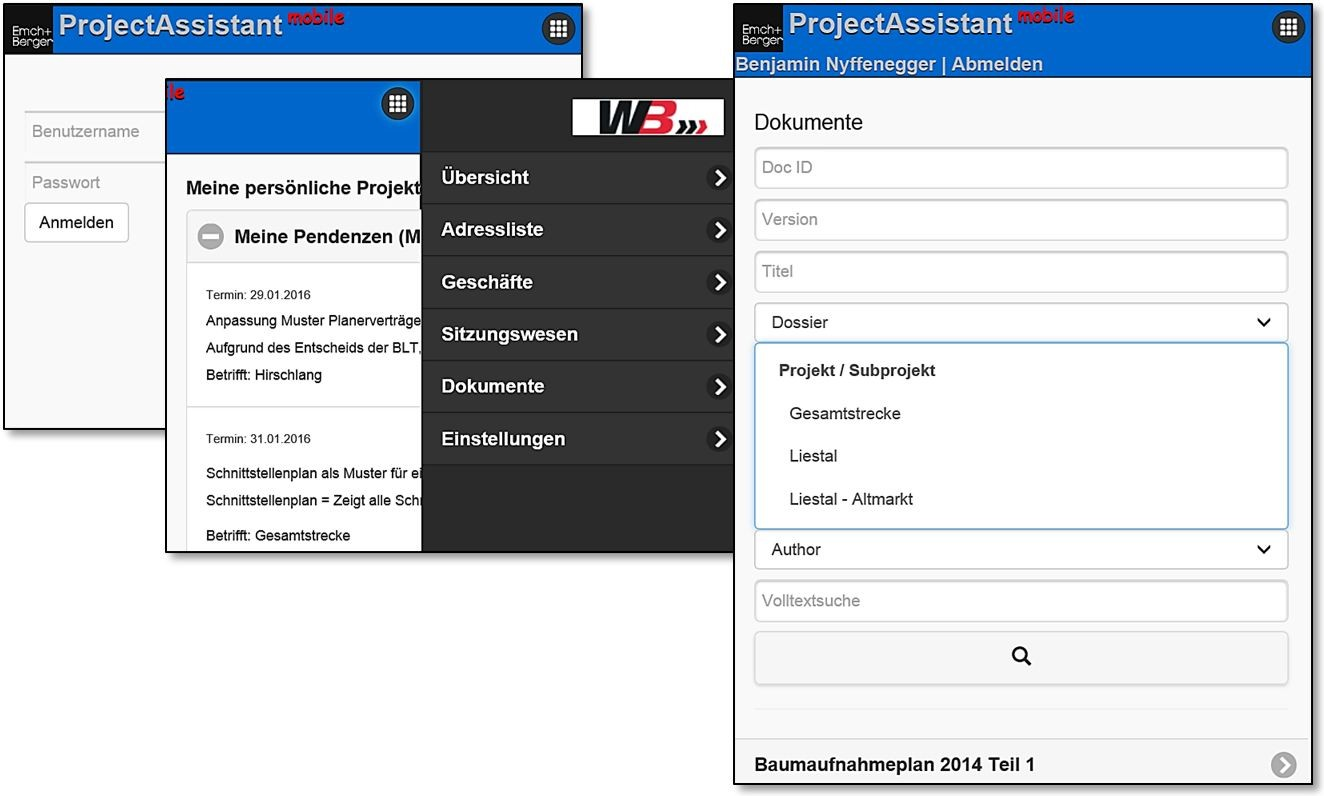
\includegraphics[width=1\linewidth]{26_Mobile_Ansicht2.jpg}}
\caption{CUBE PA - mobile view on a smartphone}
% \label{fig:speciation}
\end{figure}

The mobile view on a smartphone. Even with a smaller view, CUBE PA can be operated with touch input and can display the required information.